\documentclass[a4paper,12pt]{jsarticle}
\usepackage[dvipdfmx]{graphicx}
\usepackage{amssymb}
\usepackage{amsmath}
\usepackage{float}
\usepackage{setspace}
\usepackage{tikz}
\usetikzlibrary{decorations.pathreplacing}
\usetikzlibrary{shapes, positioning,arrows,automata,arrows.meta}
\usepackage[top=30truemm,bottom=30truemm,left=25truemm,right=25truemm]{geometry}
%---------------------------------------------------
% ページの設定
%---------------------------------------------------
% ######## measure #########
% # mm = 1mm = 2.85pt      #
% # cm = 10mm = 28.5pt     #
% # in = 25.4mm = 72.27pt  #
% # pt = 0.35mm = 1pt      #
% # em = width of [M]      #
% # ex = height of [x]     #
% # zw = width of [Kanji]  #
% # zh = height of [Kanji] #
% ##########################
% ##################### Portrait Setting #########################
% # TOP = 1inch + \voffset + \topmargin + \headheight + \headsep #
% #     = 1inch + 0pt + 4pt + 20pt + 18pt (default)              #
% # BOTTOM = \paperheight - TOP -\textheight                     #
% ################################################################
%\setlength{\textheight}{\paperheight}   % 紙面縦幅を本文領域にする(BOTTOM=-TOP)
%\setlength{\topmargin}{4.6truemm}       % 上の余白を30mm(=1inch+4.6mm)に
%\addtolength{\topmargin}{-\headheight}  % 
%\addtolength{\topmargin}{-\headsep}     % ヘッダの分だけ本文領域を移動させる
%\addtolength{\textheight}{-60truemm}    % 下の余白も30mm(BOTTOM=-TOPだから+TOP+30mm)
% #################### Landscape Setting #######################
% # LEFT = 1inch + \hoffset + \oddsidemargin (\evensidemargin) #
% #      = 1inch + 0pt + 0pt                                   #
% # RIGHT = \paperwidth - LEFT - \textwidth                    #
% ##############################################################
%\setlength{\textwidth}{\paperwidth}     % 紙面横幅を本文領域にする(RIGHT=-LEFT)
%\setlength{\oddsidemargin}{-0.4truemm}  % 左の余白を25mm(=1inch-0.4mm)に
%\setlength{\evensidemargin}{-0.4truemm} % 
%\addtolength{\textwidth}{-50truemm}     % 右の余白も25mm(RIGHT=-LEFT)
%\setlength{\textwidth}{155truemm}
%\setlength{\textheight}{235truemm}
%\setlength{\topmargin}{-6.5truemm}
%\setlength{\oddsidemargin}{2truemm}
\pagestyle{empty}
%\setlength{\headheight}{0truemm}
%\setlength{\parindent}{1zw}
\makeatletter
\def\section{\@startsection {section}{1}{\z@}{.7ex plus .2ex minus .2ex}{.1 ex plus 1.2ex}{\normalsize\bf}}
\makeatother
\setstretch{0.9}

\begin{document}
%\twocolumn[ 
\begin{center}
{\bf \Large 区間打切りデータに基づく情報量規準と感染症の潜伏期間推定への応用}
\vspace{0.3em}
\begin{tabular}{rl}
\vspace{-0.1em} \bf 神戸薬科大学, 阿部興 \\
\end{tabular}
\vspace{0.5em}
\end{center}
%]
\vspace{\baselineskip}

%\maketitle
\section{はじめに}
感染症の潜伏期間の分布は, 防疫上の様々な施策の基礎となる重要な情報である. 
しかし多くの感染症において, 発症した時点が特定される場合でも, 感染した日時が観測されることはまれであることが, 潜伏期間の分布の推定を困難にしている. 

Backer \textit{et al.} (2020) はこの問題に対する1つのアプローチを示した. 
新型コロナウイルス(COVID-19)感染症の最初の症例は, 中国の武漢で観測された. Backer \textit{et al.} (2020) は武漢への旅行者らが武漢に滞在した期間と, 発症した日のデータを用いて, 感染した時点をある種の潜在変数として扱い, 潜伏期間の分布を推定する方法を提案した. 
またその上で, leave-one-out (loo) 情報量規準を用いて, ワイブル分布, ガンマ分布, 対数正規分布を比較し, COVID-19感染症の潜伏期間に対してワイブル分布がよく適合すると論じた. 

本報告ではまず, Backer \textit{et al.} (2020) の方法が生存時間分析の分野で区間打切り(interval censored)とよばれる観測を扱う問題と等価であることを示す.  
次に, Backer \textit{et al.} (2020) の用いた方法では, loo 情報量がモデルの汎化誤差の近似としてバイアスを持ち, モデル選択の方法として妥当性が十分でないことをシミュレーションを用いて示す.

\section{観測モデルと尤度関数}
Backer \textit{et al.} (2020) は 2020年1月20日から28日に報告された88症例のデータを分析した. 
このデータにはCOVID-19感染症の患者の武漢への滞在履歴と, 発症した日が記録されている. しかし, 感染した日は未知である. 
図 \ref{concept} はこの観測の枠組みを模式的に示したものである. 

\begin{figure}[htbp]
\centering
\begin{tikzpicture}
\draw[line width=0.35mm] (0.5,0) -- (10.5,0);
\draw[line width=0.35mm] (7.0,0.25) -- (7.0,-0.25) node[above right=10pt]{発症};
\node[fill=black,draw=black,circle,inner sep=2pt,label=below:{暴露開始}] at (1,0) {};
\node[fill=white,draw=black,circle,inner sep=2pt,label=below:{感染 $s_i$}] at (3.5,0) {};
\node[fill=black,draw=black,circle,inner sep=2pt,label=below:{暴露終了}] at (6.0,0) {};
\draw [thick,decorate,decoration={brace,amplitude=6pt,raise=0pt}] (1,0.75) -- (5.9,0.75)  node [above left=8pt] {暴露の期間 $u_i$};
\draw [thick,decorate,decoration={brace,amplitude=6pt,raise=0pt}] (6.0,0.75) -- (7.0,0.75);
\node [label=above:{$t_i$}] at (6.5,1){};
\end{tikzpicture}
\caption{本報告で扱う観測}
\label{concept}
\end{figure}

本報告においては, 武漢への滞在をリスク因子への暴露とみなす. 患者 $i$ が発症した日を原点 0 とし, 原点からさかのぼり, 暴露が終了した日を $t_i$ 日前とする.  暴露の終了から $s_i$ 日前を感染した日とする. 暴露していた期間を $u_i$ とする.

この記法のもとで, 仮に $s_i$ についての完全な観測が得られた場合,  発症までの待ち時間の確率密度は $f(s_i + t_i)$ である. ここで $f(x)$ は確率密度関数とした.

Backer \textit{et al.} は, 確率密度関数 $f(x)$ にワイブル分布, ガンマ分布, および対数正規分布を選び, $s_i$ に区間 $[0, u_i]$ の一様事前分布を採用することで, $f(x)$ のパラメータと $s_i$ をあわせて推定した. この推定方法を以下では Backer 型推定と呼ぶことにする. 

一方, 古典的な生存時間分析の枠組みでは, 多くの場合, イベントの生起した時点 $s_i$ を明示的に扱うことはせずに, 密度関数を区間全体に渡って積分することで尤度関数を構成して分布を推定する (Turnbull, 1976) .  この方法を Turnbull 型推定と呼ぶことにする. 

$s_i$ を積分消去する場合,  尤度を構成する因子の患者 $i$ に関する部分は $\int_0 ^{u_i} f(s_i+t_i) \,ds_i$ である.
$x_i = s_i + t_i$ と改めておくと, この積分は $\int_{t_i} ^{u_i+t_i} f(x_i) \,dx_i$ と書き換えられる. これは Turnbull (1976) が論じた区間打切りデータに基づく尤度と同じである. 

パラメトリックに分布を推定する場合, 本報告で分析対象とするデータには3つの異なる観測があることに注意が必要である.
第1は区間が1点からなる場合, すなわち $u_i= 0$ となる場合である. 
この場合尤度を構成する因子 $L_i$ は確率密度関数そのものとなる. 
\begin{align}
L_i = f(t_i).
\end{align}

第2の観測は区間の長さ $u_i$ が有限の正の実数のときである.
この場合尤度を構成する因子 $L_i$ は次のようになる. 
\begin{align}
L_i = F(u_i+t_i) - F(t_i).
\end{align}
ここで $F(x)$ は $f(x)$ と対応する分布関数である. 

第3の観測は区間の右端が不明なときである. 
この場合, $u_i$ が無限大となるので, 尤度を構成する因子 $L_i$ は次のようになる. 
\begin{align}
L_i = 1 - F(t_i).
\end{align}

結果として, パラメータ推定のための尤度関数は(1)-(3)式の因子をすべてかけあわせたものとなる.

注意すべき点として, 第3の観測の場合を Backer 型推定では扱うことができない. Backer \textit{et al.} (2020)では $u_i$ に適当な大きな数を与えることで推定を行っている. 

\section{情報量規準}

まず loo 情報量の定義を述べる. 
事前分布の密度関数を $\phi(\theta)$ とする. また評価の対象となる確率モデルの密度関数を $p(x|\theta)$ とし, 事後分布の密度関数を $\phi^*(\theta)$とする. ここで $\theta$ はすべての未知パラメータである. 
得られたサンプル $x_1, x_2, \ldots, x_n$ から1つのサンプル $x_k$ を除いてできるデータから実現された事後分布の確率密度は, 独立同分布の仮定の下で, 
\begin{align*}
\phi^*_k(\theta) =
\frac
{\phi(\theta) \prod_{i\ne k} p(x_i| \theta)}
{\int \phi(\theta)\prod_{i\ne k} p(x_i| \theta)\,d\theta}
\end{align*}
と表わされる.
このとき, loo 情報量は次のように定義される.
\begin{align*}
\operatorname{LOOIC} =-\sum_{k=1}^n \log \left( \int p(x_k|\theta)\phi^*_k(\theta)\,d\theta \right) .
\end{align*}
この定義は次のように変形できる.
\begin{align*}
\operatorname{LOOIC} &= -\sum_{k=1}^n \log\left( 
\frac
{\int \phi(\theta)p(x_k|\theta)\prod_{i\ne k} p(x_k|\theta)\,d\theta}
{\int \phi(\theta)\prod_{i\ne k} p(x_i | \theta)\,d\theta} \right)
\\ &= -\sum_{k=1}^n  \log\left(
\frac
{\int \phi(\theta)\prod_{i=1}^n p(x_i | \theta)\,d\theta}
{\int \phi(\theta)p(x_i|\theta)^{-1}\prod_{i=1}^n p(x_i| \theta)\,d\theta}
\right)
\\ &= \sum_{k=1}^n \log\left(
\frac
{\int \phi(\theta)p(x_k|\theta)^{-1}\prod_{i=1}^n p(x_i|\theta)\,d\theta}
{\int \phi(\theta)\prod_{i=1}^n p(x_i | \theta)\,d\theta}
\right)
\\ &=\sum_{k=1}^n\log \left( \int p(x_k|\theta)^{-1} \phi^*(\theta) \, d \theta\right)
\end{align*}
この等式はサンプル1つあたりの尤度の逆数を事後分布により平均したもので, loo 情報量が計算できることを示している. 

loo 情報量は汎化損失の近似となることが知られている(渡辺, 2012).  
汎化損失は次の式で定義される. 
\begin{align*}
\operatorname{GE} = -\int q(x) \log p(x) \,dx.
\end{align*}
ここで $q(x)$ はデータを生成した分布, $p(x)$ は予測分布の密度関数である.
汎化損失は次のように変形できる.
\begin{align*}
\operatorname{GE} = \int q(x) \log \frac{q(x)}{p(x)} \,dx-\int q(x) \log q(x) \,dx.
\end{align*}
第1項は $q(x)$ と $p(x)$ のカルバック・ライブラ情報量である. 第2項はデータを生成した分布 $q(x)$ のみによって定まる量(エントロピー)であるから, 予測分布 $p(x)$ の選び方に依存しない.  すなわち, 汎化損失が小さいほどデータを生成した分布に近い予測分布が得られていると判断することができる.

一般にデータを生成した分布は未知であるから, 汎化損失を直接計算することができない. そのため, loo 情報量規準が汎化損失の近似となることは重要である.

\section{シミュレーション}

この節では Turnbull 型推定と Backer 型推定について, loo 情報量のバイアスをシミュレーションによって評価する. ここではバイアスとはloo 情報量と汎化損失の差を指す. 

Backer \textit{et al.} (2020)に習い, すべてのパラメータの事前分布に一様分布(フラットプライヤ)を採用し, 事後分布の実現には確率的プログラミング言語 Stan を用いた.

シミュレーションの設定は次の通りである. 
データを生成する分布としてワイブル分布を用い, 形状パラメータと尺度パラメータをともに2とした. 
評価の対象となるモデルとしての確率分布にもワイブル分布を用いた.
区間打切りは生成したデータの小数点以下を切り落とすことにより, 人工的に生成した. 小数点以下を切り落とすとは, 例を上げると 1.5 という乱数が生成された場合, これを区間 $[1, 2]$ の区間打切りデータとして扱うという意味である. シミュレーションの試行回数は100回とし, サンプルサイズは $n = 25,  50, 100$ と変化させた. 図 \ref{simGEplot} はこのシミュレーションの結果を示している. 図中の value は $\operatorname{GE}- \operatorname{LOOIC}/n$を意味している. 

\begin{figure}
\centering
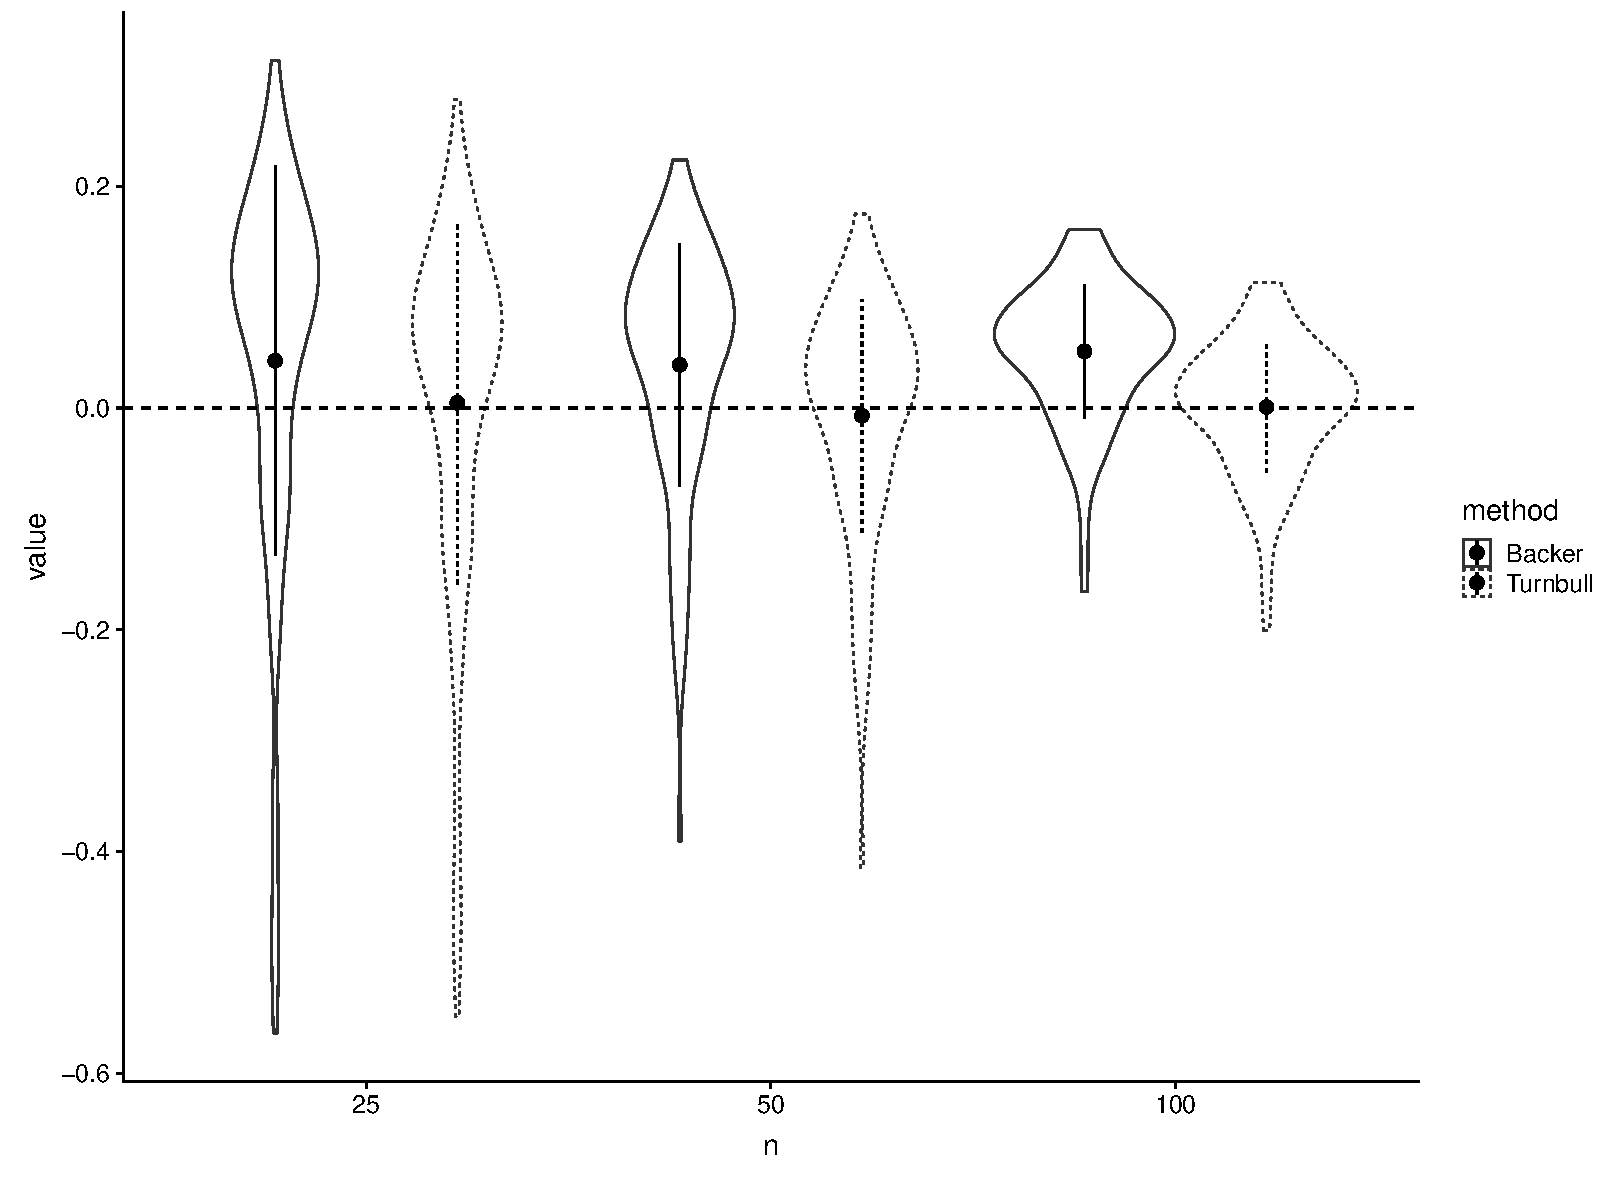
\includegraphics[width=12cm]{simGEplot.pdf}
\caption{シミュレーション結果. エラーバーは標準偏差, 点は平均を表す.}
\label{simGEplot}
\end{figure}

図 \ref{simGEplot} から, Backer 型推定では loo情報量はバイアスを持ち, そのバイアスはサンプルサイズを大きくしても小さくならないことが伺える. Turnbull 型推定はより正確に汎化損失を近似している.

\section{データ分析}

この節ではBacker \textit{et al.} (2020) と同じデータを用いて Turnbull 型推定により計算した loo 情報量と潜伏期間の予測分布を示す.

表1はモデルとしてワイブル分布, ガンマ分布, 対数正規分布を用いた場合の loo情報量である. ここでは, Backer \textit{et al.} (2020) では $\operatorname{LOOIC}$ を2倍した値を示しているため, それに習いこの表でのloo情報量は $\operatorname{LOOIC}$ の2倍を記載した.

\begin{table}[ht]
\centering
\caption{loo情報量の比較}
\begin{tabular}{lr}
  \hline
分布 & loo情報量 \\ 
  \hline
ワイブル & 73.89 \\ 
ガンマ & 73.35 \\ 
対数正規 & 73.32 \\ 
   \hline
\end{tabular}
\end{table}

表1より, Backer \textit{et al.} (2020) とは対照的に, 対数正規分布が最もよく適合するという結果が得られた. ただし対数正規分布とガンマ分布の loo 情報量の違いはごくわずかであり, MCMC の結果によって揺らぐ. 

図\ref{survfit}に上述した3つのモデルによる予測分布の生存関数を示す. 

\begin{figure}
\centering
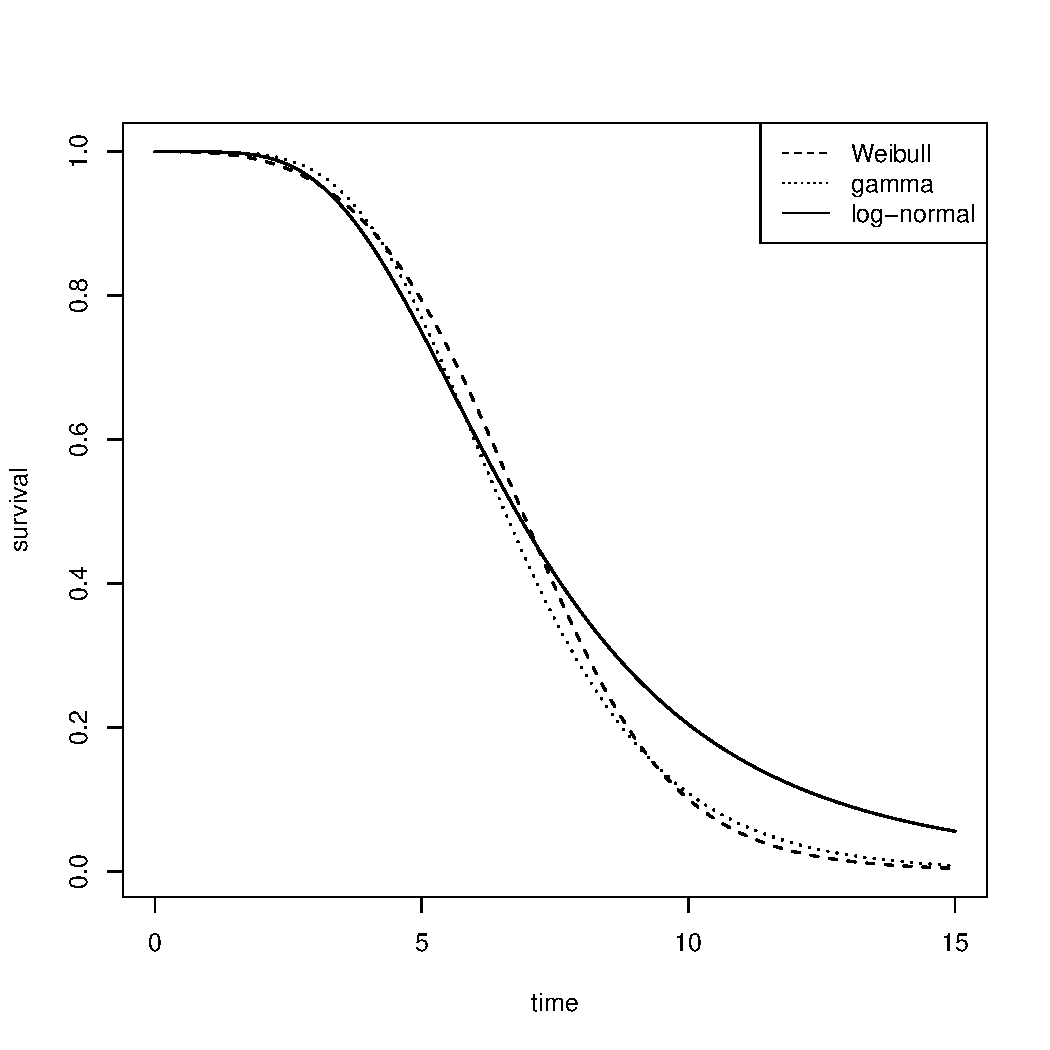
\includegraphics[width=12cm]{survfit.pdf}
\caption{潜伏期間の生存関数}
\label{survfit}
\end{figure}

図\ref{survfit}より, この場合対数正規分布が最も裾の重い予測を与えることがわかる.

また潜伏期間の95\%予測区間を表2に示す. 

\begin{table}[ht]
\centering
\caption{潜伏期間の予測区間}
\begin{tabular}{rrrr}
  \hline
 & 2.5\% & 50\% & 97.5\% \\ 
  \hline
ワイブル & 2.52 & 6.86 & 12.11 \\ 
ガンマ & 2.97 & 6.55 & 12.89 \\ 
対数正規 & 2.66 & 6.78 & 18.99 \\ 
   \hline
\end{tabular}
\end{table}

COVID-19感染症の潜伏期間は, Backer \textit{et al.}(2020) が推定したものよりも長い可能性が考えられる.

\begin{thebibliography}{9}
\bibitem{} Backer, J. A., Klinkenberg, D., \& Wallinga, J. (2020). Incubation period of 2019 novel coronavirus (2019-nCoV) infections among travellers from Wuhan, China, 20-28 January 2020. \textit{Eurosurveillance}, 25(5), 2000062.
\bibitem{} Turnbull, B. W. (1976). The empirical distribution function with arbitrarily grouped, censored and truncated data. Journal of the Royal Statistical Society: Series B (Methodological), 38(3), 290-295.
\bibitem{} 渡辺澄夫 (2012). \textbf{ベイズ統計の理論と方法.} コロナ社.
%\bibitem{} Vehtari, A., Gelman, A., \& Gabry, J. (2017). Practical Bayesian model evaluation using leave-one-out cross-validation and WAIC. Statistics and computing, 27(5), 1413-1432.
\end{thebibliography}
\end{document}  